\chapter{Resultat}\label{cha:Research}

Figure \ref{fig:evaluation} contains some preliminary evaluation results. The gray configurations in Figure \ref{fig:configurations} have not been trained yet. Each configuration takes about 15 hours to train. Still missing possibility to train on Synthia and also random data augmentations, L1 loss on disparity and velocity supervision loss.

\begin{figure}[H]
	\centering
	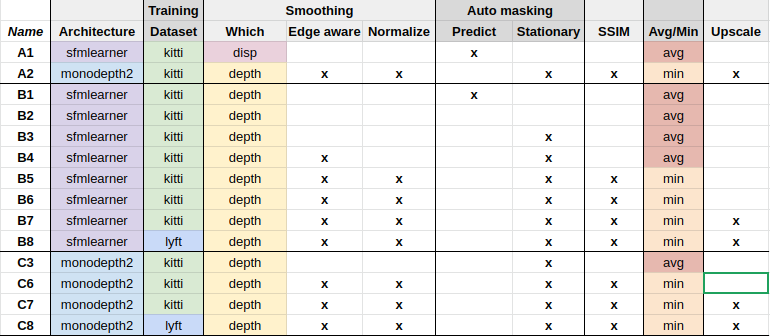
\includegraphics[width=1.0\textwidth]{configurations}
	\caption{Different configurations of network architecutes, training datasets and loss terms evaluated to find the best performance}
	\label{fig:configurations}
\end{figure}

\begin{figure}[H]
	\centering
	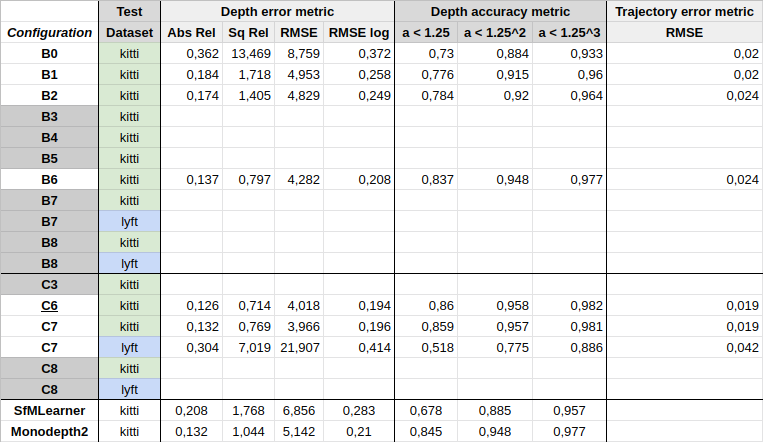
\includegraphics[width=1.0\textwidth]{evaluation}
	\caption{Evaluation metrics when testing the configurations on the testing split of the datasets}
	\label{fig:evaluation}
\end{figure}

\clearpage

\begin{figure}[H]
	\centering
	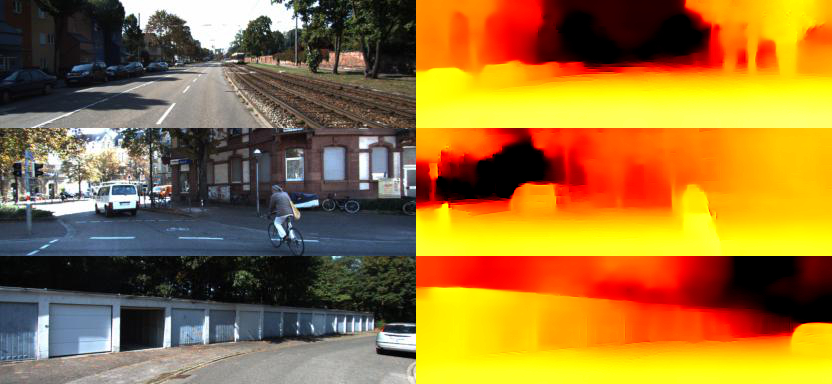
\includegraphics[width=1.0\textwidth]{depthmaps}
	\caption{Examples from the Kitti dataset}
	\label{fig:depthmapskitty}
\end{figure}

%\begin{figure}[H]
%	\centering
%	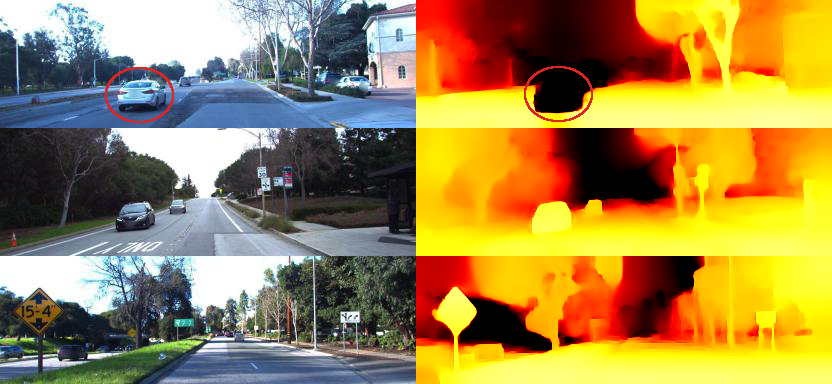
\includegraphics[width=1.0\textwidth]{depthmapslyft}
%	\caption{Examples from the Lyft dataset}
%	\label{fig:depthmaplyft}
%\end{figure}

\begin{figure}[H]
	\centering
	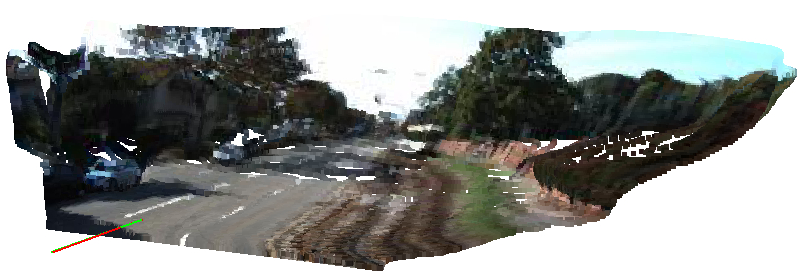
\includegraphics[width=0.8\textwidth]{3drender}
	\caption{3D render of colorized depth map}
	\label{fig:3drender}
\end{figure}

\begin{figure}[H]
	\centering
	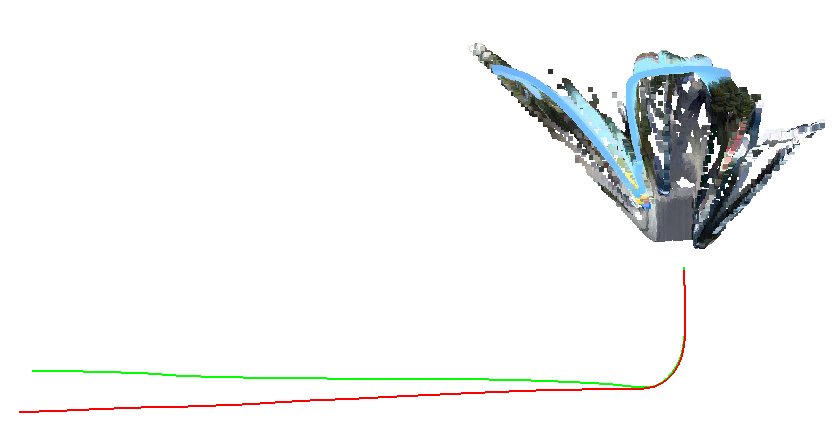
\includegraphics[width=0.8\textwidth]{movement}
	\caption{3D visualization of the camera movement in a long image sequence. The green line is ground truth and the red line is the predicted camera trajectory.}
	\label{fig:movement}
\end{figure}